\documentclass[twoside,twocolumn]{article}

\usepackage{blindtext} 
\usepackage{graphicx}
\usepackage[sc]{mathpazo} 
\usepackage[T1]{fontenc} 
\linespread{1.05} 
\usepackage{microtype} 


\usepackage[english]{babel} 


\usepackage[hmarginratio=1:1,top=32mm,columnsep=20pt]{geometry} 
\usepackage[hang, small,labelfont=bf,up,textfont=it,up]{caption} 
\usepackage{booktabs} 


\usepackage{lettrine} 


\usepackage{enumitem} 
\setlist[itemize]{noitemsep} 


\usepackage{abstract} 
\renewcommand{\abstractnamefont}{\normalfont\bfseries} 
\renewcommand{\abstracttextfont}{\normalfont\small\itshape} 


\usepackage{titlesec} 
\renewcommand\thesection{\Roman{section}} % 
\renewcommand\thesubsection{\roman{subsection}} 
\titleformat{\section}[block]{\large\scshape\centering}{\thesection.}{1em}{} 
\titleformat{\subsection}[block]{\large}{\thesubsection.}{1em}{} 


\usepackage{fancyhdr} 
\pagestyle{fancy} 
\fancyhead{} 
\fancyfoot{} 
\fancyhead[C]{Inmon vs Kimball $\bullet$ Octubre 2019 $\bullet$ } 
\fancyfoot[RO,LE]{\thepage} 


\usepackage{titling} 


\usepackage{hyperref} 


%----------------------------------------------------------------------------------------
%	TILULOS
%----------------------------------------------------------------------------------------


\setlength{\droptitle}{-4\baselineskip} 

\pretitle{\begin{center}\Huge\bfseries} 
\posttitle{\end{center}} 
\title{Inmon vs Kimball} 
\author{Andre Sebastian Reinoso Aranda
 \and Orlando Antonio Acosta Ortiz \and Arlyn Alejandra Cotrado Coaquira \and Jhony José Mamani Limache \and Roberto Carlos Zegarra Reyes
}
\date{\today} 
\renewcommand{\maketitlehookd}{

\begin{abstract}
\noindent 
Un Data WareHouse, almacen de datos, una coleccion de datos aorientada a un determinado contexto y ambito (empresas, instituciones, organizaciones, etc.). integro, no volatil y que puede cambiar en el tiempo. El principal objetivo es el de ayudar a las empresas, instituciones, organizaciones, etc. Que ayuda a tomar decisiones en la entidad quien la utilizara. Siempre a base del historial de las operaciones de la entidad que son almacenadas en una base de datos diseñada a favorecer el analisis, propagacion de los datos, con herramientas.
Por lo general las empresas medianas y grandes los datos provienen de diferentes sistemas que posee la entidad y lo que busca el Data WareHouse es unificarlas y poder operar sobre ellas con la finalidad de buscar la buena toma de decisiones.

\end{abstract}


\begin{abstract}
\noindent 
A Data WareHouse,a collection of data oriented to a certain context and scope (companies, institutions, organizations, etc.). Integral, not volatile and that can change over time. The main objective is to help companies, institutions, organizations, etc. That helps to make decisions in the entity that will use it. Always based on the history of the operations of the entity that are stored in a database designed to favor the analysis, the propagation of the data, with tools.
In general, medium and large companies, the data comes from different systems that the entity has and what Data WareHouse seeks is to unify and operate in them to seek a good decision making.
\end{abstract}
}

%----------------------------------------------------------------------------------------

\begin{document}

% Print the title
\maketitle

%----------------------------------------------------------------------------------------
%	INTRODUCCION
%----------------------------------------------------------------------------------------

\section{Introduccion}
\lettrine[nindent=0em,lines=3]{E}n la actualidad el mundo de los negocios plantea la necesidad de disponer de un acceso rápido y sencillo a información para la toma de decisiones. Dicha información debe estar estructurada y elaborada de acuerdo a parámetros de calidad, a fin de posibilitar una adaptación ágil y precisa a las fluctuaciones del ambiente externo.
Los niveles gerenciales necesitan a menudo tomar decisiones de alto nivel, cruciales para el funcionamiento de la empresa. Frecuentemente se basan en su experiencia este enfoque no es apto para las condiciones del mundo actual en el que los sistemas de gestión de calidad vigentes han demostrado la importancia de la toma de decisiones basada en cifras, datos y hechos. El Data Warehouse permite que los gerentes tomen decisiones siguiendo un enfoque racional, basados en información confiable y oportuna. Es tarea fundamental del Data Warehouse recolectar, unificar y depurar los datos del negocio, eliminando inconsistencias y conservando sólo la información útil para los objetivos empresariales.



%----------------------------------------------------------------------------------------
%	Objetivos
%----------------------------------------------------------------------------------------


\section{Objetivos}

\begin{itemize}
\item Entender la importancia del Data WareHouse en las empresas, orgnizaciones, entidades, instituciones, etc.
\item Desarrollar los antecedentes de las metodologias descritas por William H. Inmon y Ralph Kimball.
\item Comparativo de las metodologias descritas por William H. Inmon y Ralph Kimball.

\end{itemize}


%----------------------------------------------------------------------------------------
%	Marco teorico
%----------------------------------------------------------------------------------------


\section{Antecedentes}

\begin{enumerate}

 \item \textbf{William H. Inmon}
\\
William H. Inmon, científico informático estadounidense, reconocido por muchos como el padre del Data WareHouse Inmon escribió el primer libro, celebró la primera conferencia, escribió la primera columna en una revista y fue el primero en ofrecer clases del Data WareHouse. Inmon creó la definición aceptada de lo que es un Data WareHouse: una recopilación de datos variada de tiempo, no volátil, integrada y orientada al tema, en apoyo de las decisiones de la gerencia. En comparación con el enfoque del otro arquitecto pionero del almacenamiento de datos, Ralph Kimball, el enfoque de Inmon a menudo se caracteriza como un enfoque de arriba hacia abajo.
\\ 

\item \textbf{Ralph Kimball}
\\
Ralph Kimball  un autor sobre el tema del almacenamiento de datos y la inteligencia empresarial. Es uno de los arquitectos originales del almacenamiento de datos y es conocido por sus convicciones a largo plazo de que los almacenes de datos deben estar diseñados para ser comprensibles y rápidos. Su metodología, también conocida como modelado dimensional o la metodología Kimball, se ha convertido en el estándar de facto en el área de soporte de decisiones.

\end{enumerate}

%----------------------------------------------------------------------------------------
%	DESAROLLO
%----------------------------------------------------------------------------------------

\section{DESARROLLO}
\begin{enumerate}
 \item \textbf{¿Que es un Data Warehouse?}\\
Area de almacenamiento donde todos los datos de la empresa se guardan en un solo lugar. Esto incluye datos de diferentes fuentes, así como datos actuales e históricos, tal vez de una plataforma heredada.\\ \\
Puede consistir en datos de la propia empresa, que si la empresa es grande podría extenderse a muchos departamentos, todos los cuales pueden estar utilizando diferentes formatos y diferentes plataformas. Sin mencionar los datos de fuentes externas, ya sea de otras empresas o de contenido generado por el usuario.[2]

 \item \textbf{¿Que es un Data Mart?} \\
Estructura de datos, construido dentro de una base de datos este almacena información agregada o consolidada, que será consumida por alguna herramienta de visualización o data analytics. generalmente Datamart se especializa en un área de la empresa o de un flujo o proceso especifico. \\

Un Datamart almacenara la información proveniente de uno o más orígenes de datos (bases de datos, archivos con datos, servicios de internet, etc.) y que ha sido procesada por un ETL (proceso de Extracción, Transformación y Carga).\\

El Datamart contiene información consolidada, se actualiza periódicamente.

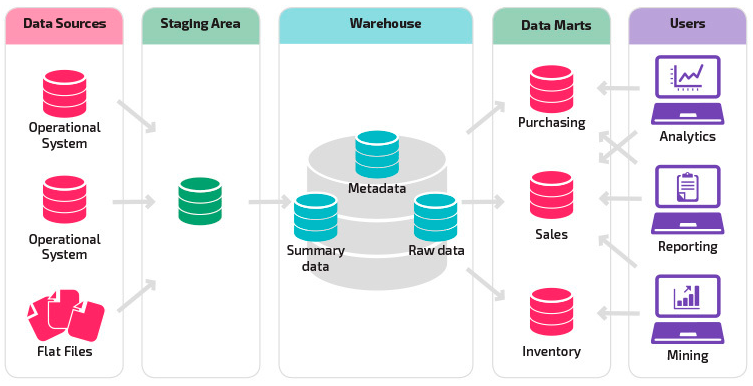
\includegraphics[width=7cm, height=5cm]{Imagenes/datawarehouse_datamart}

 \item \textbf{Enfoque Inmon}

Bill Inmon ve la necesidad de transferir la información de los diferentes OLTP (Sistemas Transaccionales) de las organizaciones a un lugar centralizado donde los datos puedan ser utilizados para el analisis (sería el CIF o Corporate Information Factory).\\

Insiste ademas en que ha de tener las siguientes características:

\textbf{Orientado a temas} Los datos en la base de datos están organizados de manera que todos los elementos de datos relativos al mismo evento u objeto del mundo real queden unidos entre sí.
\\ \\
\textbf{Integrado} La base de datos contiene los datos de todos los sistemas operacionales de la organización, y dichos datos deben ser consistentes.
\\ \\
\textbf{No volátil} La información no se modifica ni se elimina, una vez almacenado un dato, éste se convierte en información de sólo lectura, y se mantiene para futuras consultas.
\\ \\
\textbf{Variante en el tiempo} Los cambios producidos en los datos a lo largo del tiempo quedan registrados para que los informes que se puedan generar reflejen esas variaciones.
\\ \\
La información ha de estar a los máximos niveles de detalle. Los Dw departamentales o datamarts son tratados como subconjuntos de este Dw corporativo, que son construidos para cubrir las necesidades individuales de analisis de cada departamento, y siempre a partir de este Dw Central (del que también se pueden construir los ODS ( Operational Data Stores ) o similares).

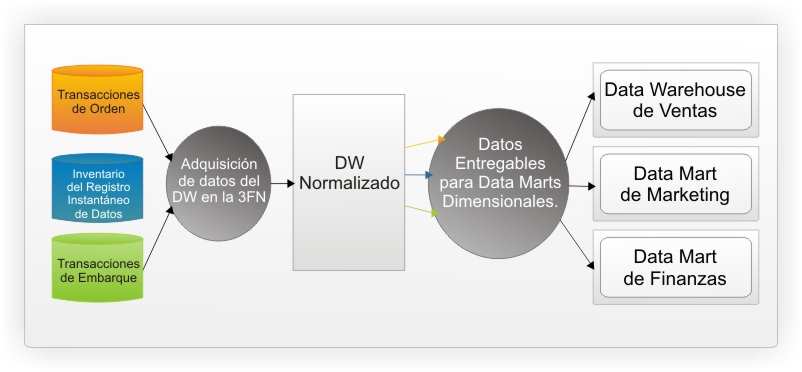
\includegraphics[width=7cm, height=5cm]{Imagenes/enfoque-inmon}

El enfoque Inmon tambien se referencia normalmente como Top-down. Los datos son extraidos de los sistemas operacionales por los procesos ETL y cargados en las areas de stage, donde son validados y consolidados en el DW corporativo, donde ademas existen los llamados metadatos que documentan de una forma clara y precisa el contenido del DW. Una vez realizado este proceso, los procesos de refresco de los Data Mart departamentales obtienen la información de el, y con las consiguientes transformaciones, organizan los datos en las estructuras particulares requeridas por cada uno de ellos, refrescando su contenido.

 \item \textbf{Enfoque Kimball}\\
El Data Warehouse es un conglomerado de todos los Data Marts dentro de una empresa, siendo una copia de los datos transaccionales estructurados de una forma especial para el analisis, de acuerdo al Modelo Dimensional (no normalizado), que incluye, como ya vimos, las dimensiones de análisis y sus atributos, su organización jerarquica, asi como los diferentes hechos de negocio que se quieren analizar. Por un lado tenemos tablas para las representar las dimensiones y por otro lado tablas para los hechos (las facts tables).
\\ \\
Los diferentes Data Marts estan conectados entre si por la llamada bus structure, que contiene los elementos anteriormente citados a traves de las dimensiones conformadas (que permiten que los usuarios puedan realizar querys conjuntos sobre los diferentes data marts, pues este bus contiene los elementos en común que los comunican). Una dimensión conformada puede ser, por ejemplo, la dimensión cliente, que incluye todos los atributos o elementos de analisis referentes a los clientes y que puede ser compartida por diferentes data marts (ventas, pedidos, gestión de cobros, etc).
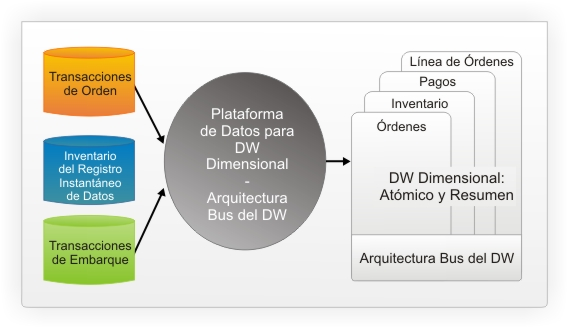
\includegraphics[width=7cm, height=5cm]{Imagenes/enfoque-kimball}
\\
   Este enfoque también se referencia como Bottom-up, pues al final el Datawarehouse Corporativo no es mas que la unión de los diferentes datamarts, que estan estructurados de una forma común a través de la bus structure. Esta caracteristica le hace mas flexible y sencillo de implementar, pues podemos construir un Data Mart como primer elemento del sistema de análisis, y luego ir añadiendo otros que comparten las dimensiones ya definidas o incluyen otras nuevas. En este sistema, los procesos ETL extraen la información de los sistemas operacionales y los procesan igualmente en el area stage, realizando posteriormente el llenado de cada uno de los Data Mart de una forma individual, aunque siempre respetando la estandarizacion de las dimensiones (dimensiones conformadas).

 \item \textbf{Ciclo de Vida Kimball}\\
Este ciclo de vida del proyecto de DW, está basado en cuatro principios básicos:\\ \\
\textbf{Centrarse en el negocio:} Hay que concentrarse en la identificación de los requerimientos del negocio y su valor asociado, y usar estos esfuerzos para desarrollar relaciones sólidas con el negocio, agudizando el análisis del mismo y la competencia consultiva de los implementadores. \\ \\
\textbf{Construir una infraestructura de información adecuada:} Diseñar una base de información única, integrada, fácil de usar, de alto rendimiento donde se reflejará la amplia gama de requerimientos de negocio identificados en la empresa. \\ \\
\textbf{Realizar entregas en incrementos significativos:} Crear el almacén de datos (DW) en incrementos entregables en plazos de 6 a 12 meses. Hay que usa el valor de negocio de cada elemento identificado para determinar el orden de aplicación de los incrementos.\\ \\
\textbf{Ofrecer la solución completa:} proporcionar todos los elementos necesarios para entregar valor a los usuarios de negocios. Para comenzar, esto significa tener un almacén de datos sólido, bien diseñado, con calidad probada, y accesible. \\ \\

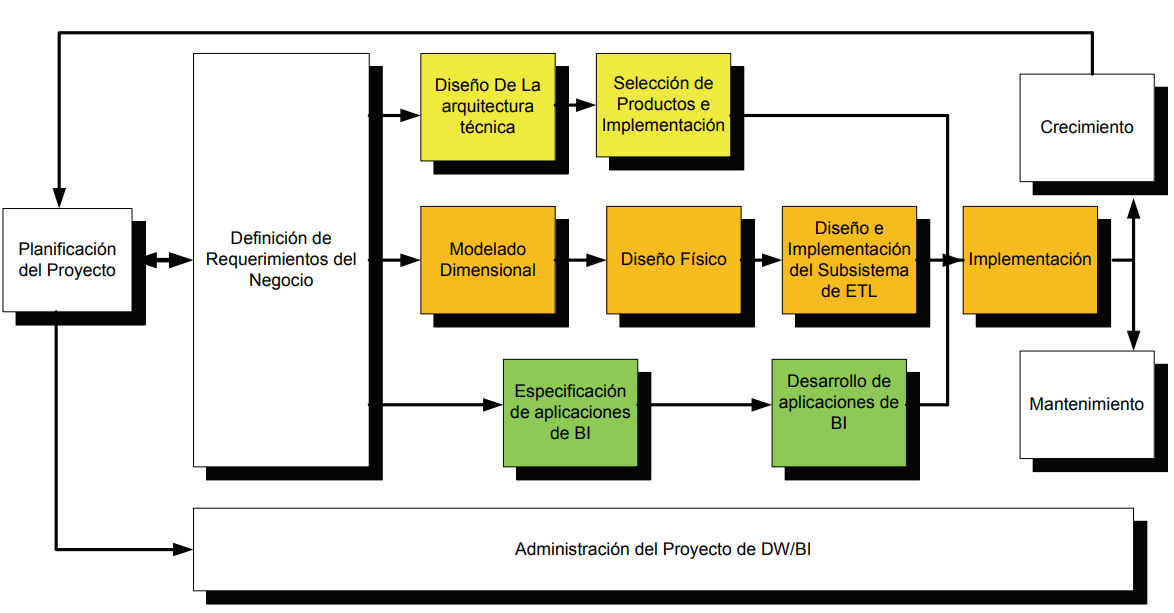
\includegraphics[width=7cm, height=5cm]{Imagenes/ciclodevidakimball}


 \item \textbf{Definicion de Requerimientos}\\
 
 La definición de los requerimientos es en gran medida un proceso
de entrevistar al personal de negocio y técnico, pero siempre conviene 
Cuadernos de la Facultad n. 5, 2010
61
tener un poco de preparación previa. Se debe aprender tanto como se
pueda sobre el negocio, los competidores, la industria y los clientes del
mismo. Hay que leer todos los informes posibles de la organización;
rastrear los documentos de estrategia interna; entrevistar a los
empleados, analizar lo que se dice en la prensa acerca de la
organización, la competencia y la industria. Se deben conocer los
términos y la terminología del negocio.
Parte del proceso de preparación es averiguar a quién se debe
realmente entrevistar. Esto normalmente implica examinar
cuidadosamente el organigrama de la organización. Hay básicamente
cuatro grupos de personas con las que hablar desde el principio: el
directivo responsable de tomar las decisiones estratégicas; los
administradores intermedios y de negocio responsables de explorar
alternativas estratégicas y aplicar decisiones; personal de sistemas, si
existen, la gente que realmente sabe qué tipos de problemas
informáticos y de datos existen; y por último, la gente que se necesita
entrevistar por razones políticas.
A partir de las entrevistas, podemos identificar temas analíticos y
procesos de negocio. Los temas analíticos agrupan requerimientos
comunes en un tema común.


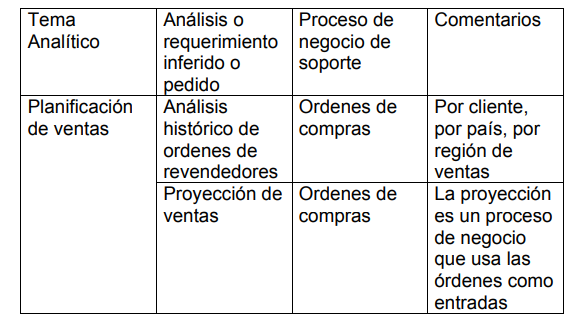
\includegraphics[width=7cm, height=5cm]{Imagenes/img}


\item \textbf{Matriz de Negocio(Bus Matrix)}\\
 
 Por otra parte, a partir del análisis se puede construir una
herramienta de la metodología denominada matriz de
procesos/dimensiones (Bus Matrix en inglés).
Una dimensión es una forma o vista o criterio por medio de cual se
pueden sumariar, cruzar o cortar datos numéricos a analizar, datos que
se denominan medidas (measures en inglés).
Esta matriz tiene en sus filas los procesos de negocio
identificados, y en las columnas, las dimensiones identificadas.
Un ejemplo de esta matriz se puede observar en la tabla. Cada
X en la intersección de las filas y columnas significa que en el proceso
de negocio de la fila seleccionada se identifican las dimensiones
propuestas.

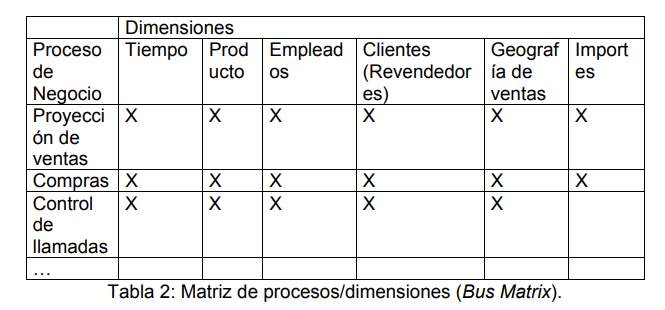
\includegraphics[width=7cm, height=5cm]{Imagenes/img2}


\item \textbf{Linea de Desarrollo}\\

hay que resaltar el rol central de la tarea de definición de requerimientos.
Los requerimientos del negocio son el soporte inicial de las tareas
subsiguientes. También tiene influencia en el plan de proyecto (nótese
la doble fecha entre la caja de definición de requerimientos y la de
planificación). En segundo lugar podemos ver tres rutas o caminos que
se enfocan en tres diferentes áreas:

\begin{itemize}
	\item \textbf{Tecnología (Camino Superior)}. Implica tareas relacionadas con
software específico, por ejemplo, Microsoft SQL Analysis Services.\\

	\item \textbf{Datos (Camino del medio)}. En la misma diseñaremos e
implementaremos el modelo dimensional, y desarrollaremos el
subsistema de Extracción, Transformación y Carga (Extract,
Transformation, and Load - ETL) para cargar el DW.\\

 	\item \textbf{Aplicaciones de Inteligencia de Negocios (Camino Inferior)} En
esta ruta se encuentran tareas en las que diseñamos y
desarrollamos las aplicaciones de negocios para los usuarios
finales. 
	
\end{itemize}

Estas rutas se combinan cuando se instala finalmente el sistema.
En la parte de debajo de la figura se muestra la actividad general de
administración del proyecto. A continuación describiremos cada una de
las tareas.

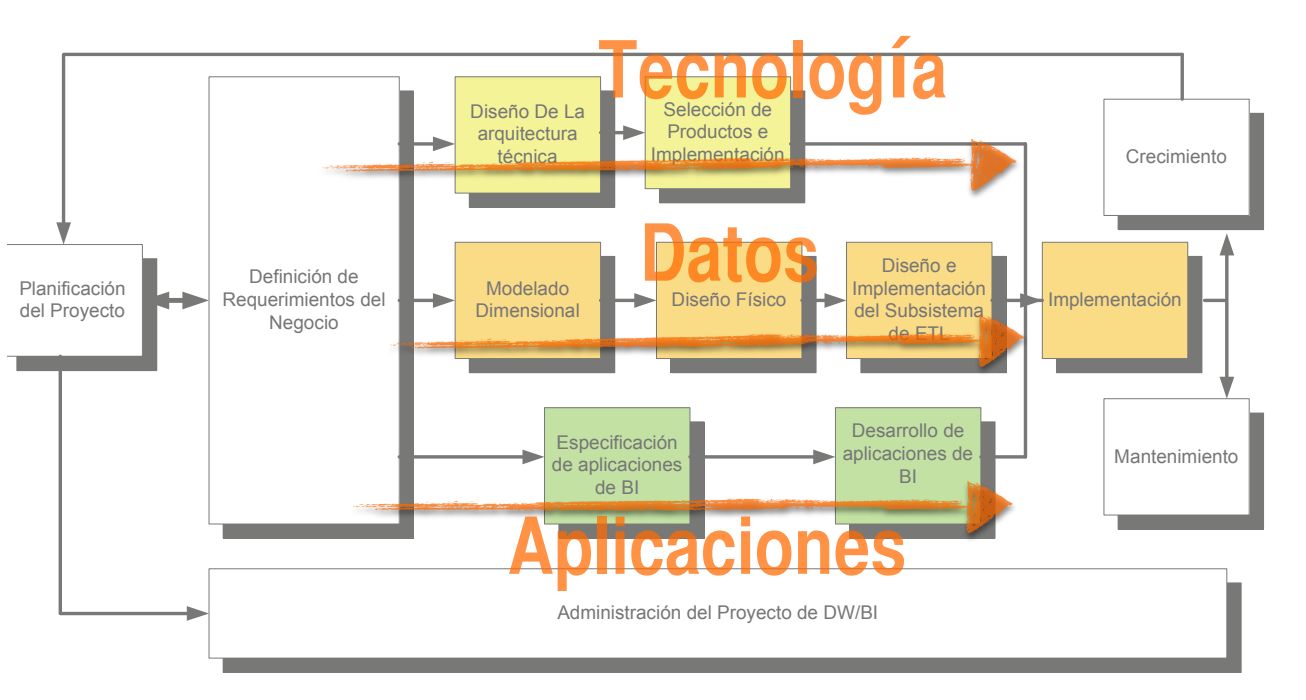
\includegraphics[width=7cm, height=5cm]{Imagenes/img3}




 \item \textbf{Linea de Datos}\\
El seguimiento de datos comienza con el diseño de un modelo dimensional objetivo para abordar los requisitos comerciales, mientras se consideran las realidades de datos subyacentes. El modelo dimensional se convierte en un diseño físico donde se consideran las estrategias de ajuste de rendimiento, luego se abordan los desafíos de diseño y desarrollo del sistema ETL.\\ \\
\textbf{Modelo dimensional:} es un proceso dinámico y altamente iterativo. Consiste de cuatro pasos:
\begin{itemize}
	\item Elegir el proceso de negocio: El primer paso es elegir el área a modelizar. Esta es una decisión de la dirección, y depende fundamentalmente del análisis de requerimientos y de los temas analíticos anotados en la etapa anterior. 
	\item Establecer el nivel de granularidad: La granularidad significa especificar el nivel de detalle. La elección de la granularidad depende de los requerimientos del negocio y lo que es posible a partir de los datos actuales.
	\item Elegir las dimensiones: Las dimensiones surgen naturalmente de las discusiones del equipo, y facilitadas por la elección del nivel de granularidad y de la matriz de procesos/dimensiones. Una forma de identificar las tablas de dimensiones es que sus atributos
son posibles candidatos para ser encabezado en los informes, tablas pivot, cubos, o cualquier forma de visualización, unidimensional o
multidimensional.
	\item Identificar medidas y tablas de hechos: El último paso consiste en identificar las medidas que surgen de
los procesos de negocios. Una medida es un atributo (campo) de una tabla que se desea analizar, sumarizando o agrupando sus datos,
usando los criterios de corte conocidos como dimensiones.
	\item Para concluir con el proceso dimensional inicial se realiza un gráfico denominado modelo dimensional de alto nivel (o gráfico de burbujas, Bubble chart, en el léxico de Kimball)
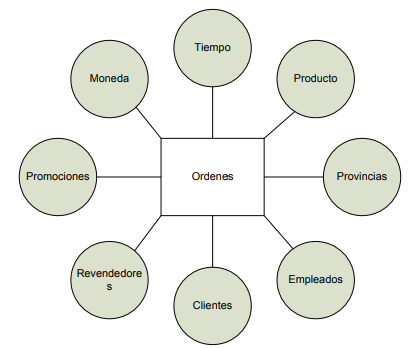
\includegraphics[width=8cm, height=6cm]{Imagenes/2}
\end{itemize}
\textbf{Modelo fisico:} En esta parte, intentamos contestar las siguientes preguntas: 
\begin{itemize}
	\item ¿Cómo puede determinar cuán grande será el sistema de DW/BI? 
	\item ¿Cuáles son los factores de uso que llevarán a una configuración más grande y más compleja? 
	\item ¿Cómo se debe configurar el sistema? 
	\item ¿Cuánta memoria y servidores se necesitan? ¿Qué tipo de almacenamiento y procesadores?
	\item ¿Cómo instalar el software en los servidores de desarrollo, prueba
y producción?
	\item ¿Qué necesitan instalar los diferentes miembros del equipo de
DW/BI en sus estaciones de trabajo?
	\item ¿Cómo convertir el modelo de datos lógico en un modelo de datos
físicos en la base de datos relacional?
	\item ¿Cómo conseguir un plan de indexación inicial?
	\item ¿Debe usarse la partición en las tablas relacionales?
\end{itemize}
\textbf{ETL:} El sistema de Extracción, Transformación y Carga (ETL) es la base sobre la cual se alimenta el Datawarehouse. Si el sistema ETL se diseña adecuadamente, puede extraer los datos de los sistemas de origen de datos, aplicar diferentes reglas para aumentar la calidad y consistencia de los mismos, consolidar la información proveniente de distintos sistemas, y finalmente cargar (grabar) la información en el DW en un formato acorde para la utilización por parte de las herramientas de análisis. 

 \item \textbf{Linea de Aplicación de BI}\\
Mientras que algunos miembros del proyecto están inmersos en la tecnología y los datos, otros se centran en identificar y construir una amplia gama de aplicaciones de BI, incluidos informes estandarizados, consultas parametrizadas, paneles, cuadros de mandos, modelos analíticos, aplicaciones de minería de datos, junto con el interfaces de navegación asociadas.

\end{enumerate}


%----------------------------------------------------------------------------------------
%	GRAFICOS
%----------------------------------------------------------------------------------------

\section{graficos}

En esta tarea se proporciona, a una gran comunidad de usuarios una forma mas estructurada y por lo tanto, mas facil, de acceder al almacen de datos. Se proporciona este acceso estructurado a traves de lo que llamamos, aplicaciones de inteligencia de negocios (BusinessIntelligence Aplications). Las aplicaciones de BI son la cara visible de la inteligencia de negocios: los informes y aplicaciones de analisis proporcionan informacion util a los usuarios. Las aplicaciones de BI incluyen un amplio espectro de tipos de informes y herramientas de analisis,que van desde informes simples de formato fijo, a sofisticadas aplicaciones analıticas que usan complejos algoritmos e informacion del dominio. Kimball divide a estas aplicaciones en dos categorıas basadas en el nivel de sofisticacion, y les llama: \\a) Informes estandar: son informes relativamente simples, de formato predefinido, y parametros de consulta fijos, proporcionan a los usuarios un conjunto basico de informacion acerca de lo que esta sucediendo en un area determinada de la empresa y se utilizan dıa a dıa. \\b) Aplicaciones analıticas: Son mas complejasque los informes estandar. Estas aplicaciones pueden incluir algoritmos y modelos de minerıade  datos,  que  ayudan  a  identificar  oportunidades  o  cuestiones  subyacentes  en  los  datos,  yel usuario puede pedir cambios en los sistemas transaccionales basandose en los conocimientos obtenidos del uso de la aplicacion de BI. . \\\\
 
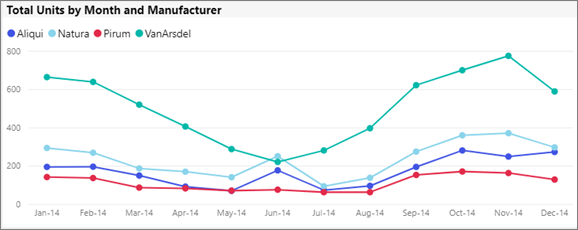
\includegraphics[width=7cm, height=5cm]{Imagenes/power-bi-line}
\\ 

   


%----------------------------------------------------------------------------------------
%	DIAGRAMAS
%----------------------------------------------------------------------------------------

\section{Análisis}



    Los análisis son el estudio de datos para encontrar información significativa y detallada. Es una aplicación muy popular entre las herramientas de inteligencia de negocios, ya que permite a las empresas comprender sus datos en profundidad y generar valor en sus decisiones basadas en datos. Por ejemplo, una empresa de marketing podría usar este análisis para determinar los segmentos de clientes que tienen más probabilidad de convertirse en nuevos clientes.
    \\ \\
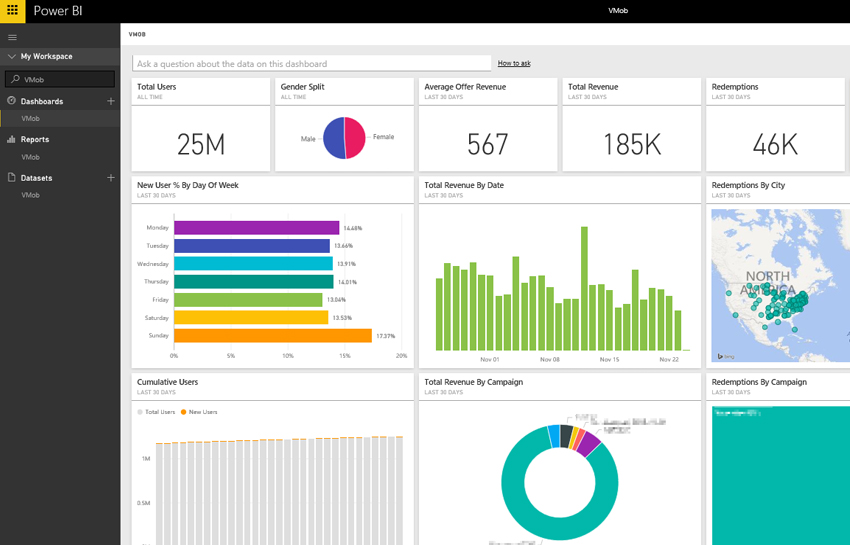
\includegraphics[width=7cm, height=5cm]{Imagenes/linea_bi1}

  \begin{enumerate}  
\item \textbf{Despliegue}
    \begin{itemize}
	    \item \textbf{Despliegue} \\
	    - debe ser sincronizado. \\
	    - Se debera aplazar si todas las piezas no estan listas para produccion
	\begin{itemize}
	    \item Entrenamiento \\
	    \item Documentacion \\
	    \item Validacion de datos \\
    \end{itemize}
    \\
    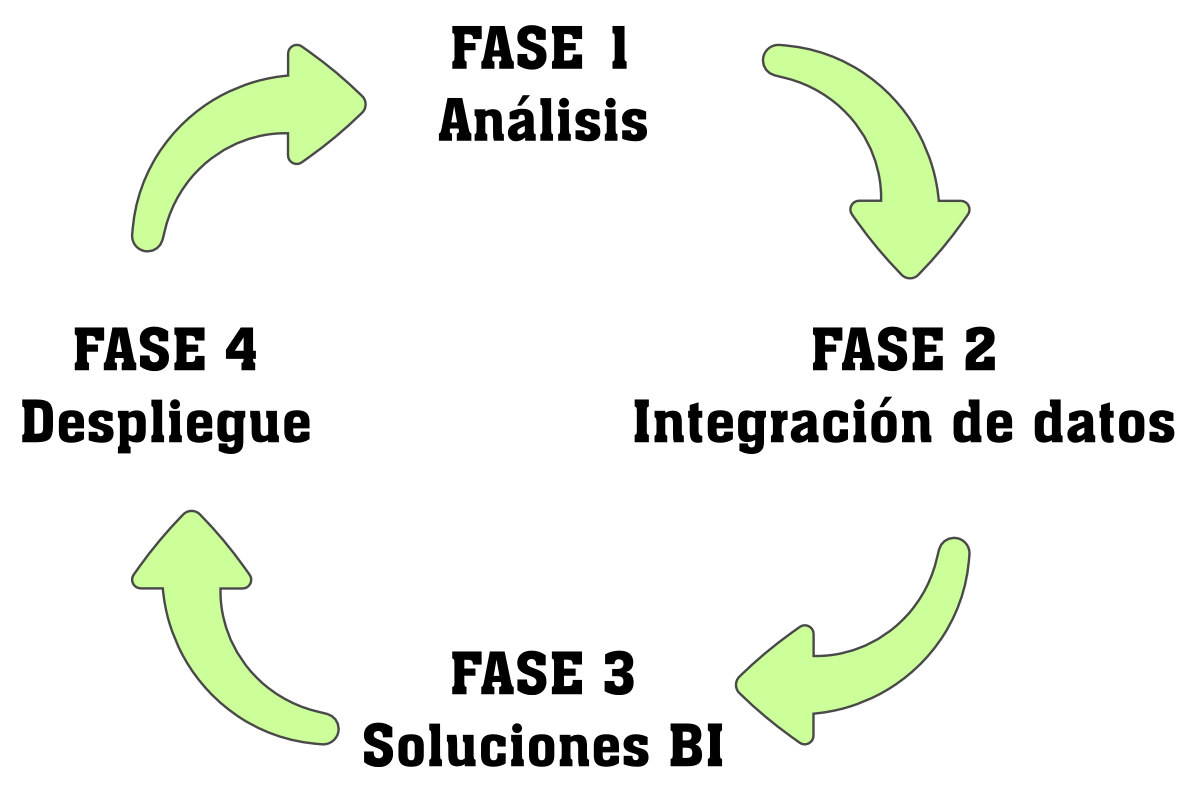
\includegraphics[width=7cm, height=5cm]{Imagenes/despliegue}
    \\\\\\\\
	\item \textbf{Mantenimiento}\\
	- cuando el sistema este en produccion.\\
	- tareas operacionales:
	\begin{itemize}
	    \item Monitoreo \\
	    \item Tunning del desempeño \\
	    \item Mantenimiento de indices \\
	    \item Backups \\
	    
	\end{itemize}
	- Apoyo permanente , capacitacion y comunicacion con los usuarios finales. \\
	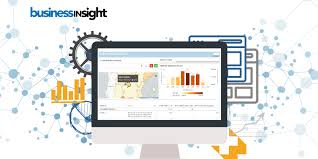
\includegraphics[width=7cm, height=5cm]{Imagenes/mantenimiento}
	\\
	\item \textbf{Crecimiento}\\
	- Los DW tienden a expandirse.\\
	- Es considerado un signo de exito.\\
	- Nuevos requerimientos deben ser prioridad.\\
	- empezar el ciclo de nuevo : \\
	\begin{itemize}
	    \item Construir sobre las bases ya establecidas.  \\
	    \item Enfoque en los nuevos Requerimientos. \\
	    
	\end{itemize}
\end{itemize}

\end{enumerate}


\includegraphics[width=7cm, height=5cm]{Imagenes/crecimiento}

%----------------------------------------------------------------------------------------
%	CONCLUSIONES
%----------------------------------------------------------------------------------------
\newpage
\section{Conclusiones}
\begin{itemize}	
\item Se ha demostrado que tanto el enfoque de Inmon como el de Kimball funcionan para entregar con éxito almacenes de datos. Incluso hay organizaciones donde se ha implementado una combinación de ambos ('modelo híbrido'). En un modelo híbrido, el almacén de datos se construye utilizando el modelo Inmon, y además del almacén de datos integrado, los almacenes de datos orientados a procesos de negocio se construyen utilizando el esquema en estrella para la presentación de informes. No podemos generalizar y decir que un enfoque es mejor que el otro; Ambos tienen sus ventajas y desventajas, y ambos funcionan bien en diferentes escenarios. El arquitecto tiene que seleccionar un enfoque para el almacén de datos en función de los diferentes factores; Se identificaron algunas claves en este documento. Finalmente, para que cualquier enfoque sea exitoso, debe ser cuidadosamente pensado, discutido en detalle. 

\end{itemize} 

\newpage

%----------------------------------------------------------------------------------------
%	BIBLIOGRAFIA
%----------------------------------------------------------------------------------------


\begin{thebibliography}{99} 

\bibitem[1]{}
\newblock W. H. Inom, 2002. Building the Data Warehouse

\bibitem[2]{}
\newblock Spotless. Exploring Data Warehouse and Data Quality, Reduperado de: web.archive.org

\bibitem[3]{}
\newblock I, Abramson, 20 IAS Inc. Data Warehouse: The Choice of Inmon versus Kimball

\bibitem[4]{}
\newblock Rivadera, G. La metodología de Kimball para el diseño de almacenes de
datos (Data warehouses) 

\end{thebibliography}


%----------------------------------------------------------------------------------------


\end{document}
